\documentclass[11pt,a4paper]{article}

% ── Packages ───────────────────────────────────────────────────────────
\usepackage[utf8]{inputenc}
\usepackage[T1]{fontenc}
\usepackage{geometry}
\geometry{margin=2.5cm}
\usepackage{amsmath,amssymb}
\usepackage{graphicx}
\usepackage{booktabs}
\usepackage{hyperref}
\usepackage{cite}
\usepackage{enumitem}
\usepackage{float}
\usepackage{caption}
\usepackage{subcaption}
\usepackage{xcolor}

\hypersetup{
    colorlinks=true,
    linkcolor=blue,
    citecolor=blue,
    urlcolor=blue,
}

\title{%
  Infant Cry Classification Using Classical Machine Learning\\[6pt]
  \large Phase~1 Report — Foundation \& Baseline Models
}
\author{Belal Raza}
\date{\today}

\begin{document}
\maketitle

% ======================================================================
\begin{abstract}
Infant cry is a primary communication channel between newborns and
caregivers, yet interpreting the underlying cause of distress remains
challenging even for experienced parents.  This project develops an
automatic classification system that maps short audio recordings of
infant cries to one of five distress categories: \textit{hunger},
\textit{belly pain}, \textit{burping}, \textit{discomfort}, and
\textit{tiredness}.  In this first phase we establish a classical
machine-learning baseline using Mel-frequency cepstral coefficients
(MFCCs) and statistical spectral features, evaluated with a Gaussian
Mixture Model (GMM), a Support Vector Machine (SVM), and an exploratory
Hidden Markov Model (HMM).  We present a full exploratory data analysis,
validate key distributional assumptions, and report per-class precision,
recall, and F1 scores.
\end{abstract}

% ======================================================================
\section{Introduction}
\label{sec:intro}

Crying is the earliest and most instinctive form of vocal communication
for human infants~\cite{dunstan2006}.  Different physiological states —
hunger, gastrointestinal discomfort, fatigue, need for burping, or
general discomfort — produce acoustically distinct cry patterns, though
the differences are subtle and easily confounded by noise, recording
conditions, and individual variation.

Automated cry classification has practical value in neonatal care,
smart-nursery devices, and developmental monitoring.  Early systems
relied on hand-crafted acoustic features and classical
classifiers~\cite{ji2021review}, while recent work has shifted toward
deep learning on spectrogram representations~\cite{chang2017infant}.
However, the interpretability and low data requirements of classical
approaches make them an important baseline, especially in settings where
labelled data is scarce.

\paragraph{Contributions of this phase.}
\begin{enumerate}[nosep]
  \item A reproducible feature-extraction pipeline based on MFCCs,
        delta coefficients, and spectral descriptors (750-dimensional
        feature vector per clip).
  \item A GMM-based generative classifier (one mixture per class) and
        an SVM-based discriminative classifier with grid-searched
        hyper-parameters.
  \item An exploratory HMM classifier that models temporal dynamics at
        the frame level.
  \item Statistical validation of stationarity (Augmented Dickey--Fuller)
        and Gaussianity (Shapiro--Wilk, D'Agostino--Pearson) assumptions
        underlying the chosen models.
\end{enumerate}

% ======================================================================
\section{Related Work}
\label{sec:related}

\subsection{Acoustic Features for Cry Analysis}

Mel-frequency cepstral coefficients (MFCCs) are the dominant feature
representation in audio classification~\cite{davis1980mfcc}.  For infant
cry analysis, MFCCs capture the spectral envelope shaped by the infant's
vocal tract, which varies with the type of distress.  Supplementary
features — zero-crossing rate (ZCR), spectral centroid, spectral
bandwidth, spectral roll-off, and root-mean-square (RMS) energy —
provide complementary information about the signal's noisiness, pitch
centre, and loudness.

Delta and delta-delta (acceleration) coefficients encode the temporal
dynamics of the spectral envelope over consecutive frames, capturing
transitions that are characteristic of specific cry
types~\cite{ji2021review}.

\subsection{Classical ML for Audio Classification}

\paragraph{Gaussian Mixture Models (GMMs).}
GMMs model each class as a mixture of multivariate Gaussians in feature
space.  At test time, a sample is assigned to the class whose GMM yields
the highest log-likelihood.  This generative approach is well-suited to
audio because the distribution of MFCC vectors within a class is often
approximately Gaussian~\cite{reynolds2000speaker}.

\paragraph{Support Vector Machines (SVMs).}
SVMs find the maximum-margin hyperplane (or, with a kernel, a nonlinear
decision surface) separating classes in feature space.  With an RBF
kernel and proper regularisation, SVMs have proven competitive on
moderate-dimensional audio features~\cite{chang2011libsvm}.

\paragraph{Hidden Markov Models (HMMs).}
HMMs extend GMMs by modelling the temporal sequence of feature frames as
a Markov chain of hidden states, each emitting observations from a
Gaussian distribution.  HMMs were the standard in speech recognition for
decades~\cite{rabiner1989hmm} and naturally capture the evolving
structure of a cry episode.

\subsection{Deep Learning Approaches (Phase~2 Preview)}

Convolutional neural networks (CNNs) applied to Mel-spectrogram images
have achieved state-of-the-art results on environmental sound
classification~\cite{hershey2017cnn}.  Recurrent architectures (LSTMs)
and attention-based models further exploit temporal structure.  These
approaches will be explored in Phase~2 of this project.

% ======================================================================
\section{Methodology}
\label{sec:methods}

\subsection{Dataset}

The dataset comprises short audio recordings of infant cries organised
into five classes: \textit{hunger}, \textit{belly\_pain},
\textit{burping}, \textit{discomfort}, and \textit{tiredness}.  Each
clip is loaded at its native sampling rate of 8\,000\,Hz and padded or
truncated to a fixed duration of 7~seconds (56\,000 samples).

\subsection{Feature Extraction}
\label{sec:features}

For each clip we extract the following features:

\begin{enumerate}[nosep]
  \item \textbf{MFCC summary} — 40 MFCCs computed with a 512-sample
        FFT window ($\approx$64\,ms at 8\,kHz) and 160-sample hop
        ($\approx$20\,ms).  Each coefficient's time series
        is summarised by six statistics: mean, standard deviation,
        minimum, maximum, skewness, and kurtosis.
        Dimensionality: $40 \times 6 = 240$.
  \item \textbf{Delta-MFCC summary} — first-order temporal derivative
        of the MFCC matrix, summarised identically.  Dim: 240.
  \item \textbf{Delta-delta-MFCC summary} — second-order derivative.
        Dim: 240.
  \item \textbf{Spectral descriptors} — ZCR, spectral centroid,
        bandwidth, roll-off, and RMS energy, each summarised by the
        same six statistics.  Dim: $5 \times 6 = 30$.
\end{enumerate}

\noindent
Total feature vector dimensionality: $\mathbf{750}$.

\subsection{Statistical Validation}

\paragraph{Stationarity.}
We apply the Augmented Dickey--Fuller (ADF) test to the raw waveform of
a random subset of clips per class.  The null hypothesis is that the
signal contains a unit root (non-stationary); a $p$-value below 0.05
leads us to reject the null and conclude the signal is stationary.
Audio signals are typically wide-sense stationary over short analysis
windows, which justifies the use of frame-based STFT and MFCC
extraction.

\paragraph{Gaussianity.}
We test whether the clip-level MFCC features within each class follow a
Gaussian distribution using the Shapiro--Wilk test (for small samples)
and the D'Agostino--Pearson omnibus test (for larger samples).
Approximate Gaussianity within classes supports the GMM modelling
assumption.

\subsection{Models}

\subsubsection{GMM Classifier}

We train one Gaussian Mixture Model per class on the 750-dimensional
feature vectors.  Each GMM uses diagonal covariance matrices and 8
mixture components (adjusted downward if a class has fewer than 8
training samples).  At inference, the class whose GMM yields the highest
per-sample log-likelihood is selected:

\begin{equation}
  \hat{y} = \arg\max_{c \in \mathcal{C}} \;
             \log p(\mathbf{x} \mid \boldsymbol{\theta}_c)
\end{equation}

\noindent
where $\boldsymbol{\theta}_c$ denotes the parameters of the GMM for
class~$c$.

\subsubsection{SVM Classifier}

We train a multi-class SVM with a radial basis function (RBF) kernel.
Features are standardised (zero mean, unit variance) before training.
Hyper-parameters $C$ and $\gamma$ are selected via 5-fold
cross-validated grid search, optimising macro-averaged F1:

\begin{equation}
  K(\mathbf{x}_i, \mathbf{x}_j) =
    \exp\!\bigl(-\gamma \|\mathbf{x}_i - \mathbf{x}_j\|^2\bigr)
\end{equation}

\subsubsection{HMM Classifier (Exploratory)}

For the HMM we use frame-level MFCC sequences (shape $T \times 40$
per clip) rather than clip-level summaries.  One left-to-right Gaussian
HMM with 5 hidden states and diagonal covariance is trained per class.
Classification follows the same maximum-likelihood rule as the GMM.

\subsection{Evaluation Protocol}

The dataset is split 80/20 (train/test) with stratification by class.
All splits use a fixed random seed for reproducibility.  We report:

\begin{itemize}[nosep]
  \item Per-class precision, recall, and F1-score.
  \item Macro-averaged and weighted-averaged F1.
  \item Overall accuracy.
  \item Normalised confusion matrices.
\end{itemize}

% ======================================================================
\section{Results}
\label{sec:results}

\textit{(To be completed after running the pipeline on the full dataset.)}

\subsection{Class Distribution}

\begin{table}[H]
\centering
\caption{Number of clips per class.}
\label{tab:class_dist}
\begin{tabular}{lc}
\toprule
\textbf{Class} & \textbf{Count} \\
\midrule
hunger     & --- \\
belly\_pain & --- \\
burping    & --- \\
discomfort & --- \\
tiredness  & --- \\
\bottomrule
\end{tabular}
\end{table}

\subsection{Model Performance}

\begin{table}[H]
\centering
\caption{Test-set performance of Phase~1 classifiers.}
\label{tab:results}
\begin{tabular}{lccc}
\toprule
\textbf{Model} & \textbf{Accuracy} & \textbf{Macro F1} & \textbf{Weighted F1} \\
\midrule
GMM & --- & --- & --- \\
SVM & --- & --- & --- \\
HMM & --- & --- & --- \\
\bottomrule
\end{tabular}
\end{table}

\subsection{Confusion Matrices}

\textit{(Figures to be inserted from} \texttt{results/plots/}\textit{.)}

% \begin{figure}[H]
% \centering
% 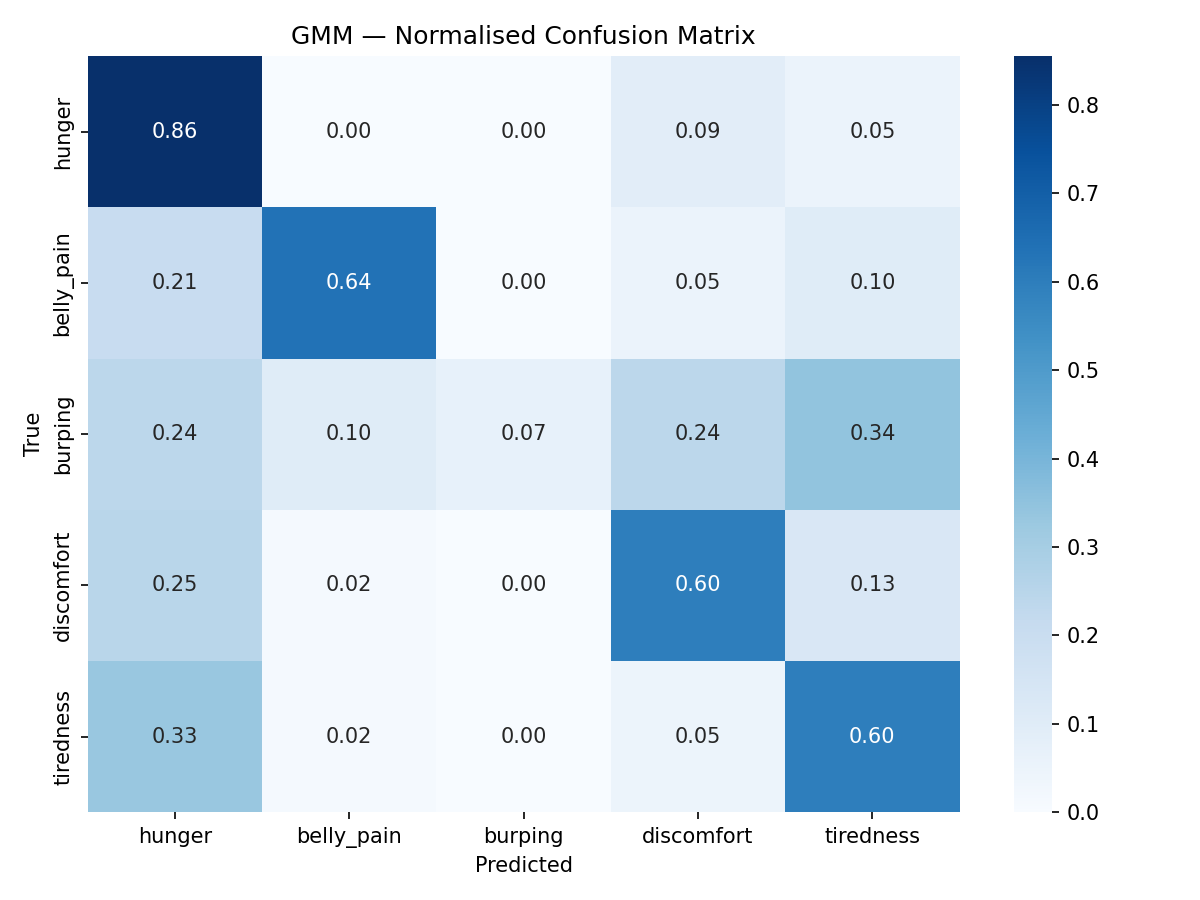
\includegraphics[width=0.48\textwidth]{../results/plots/GMM_confusion_matrix.png}
% 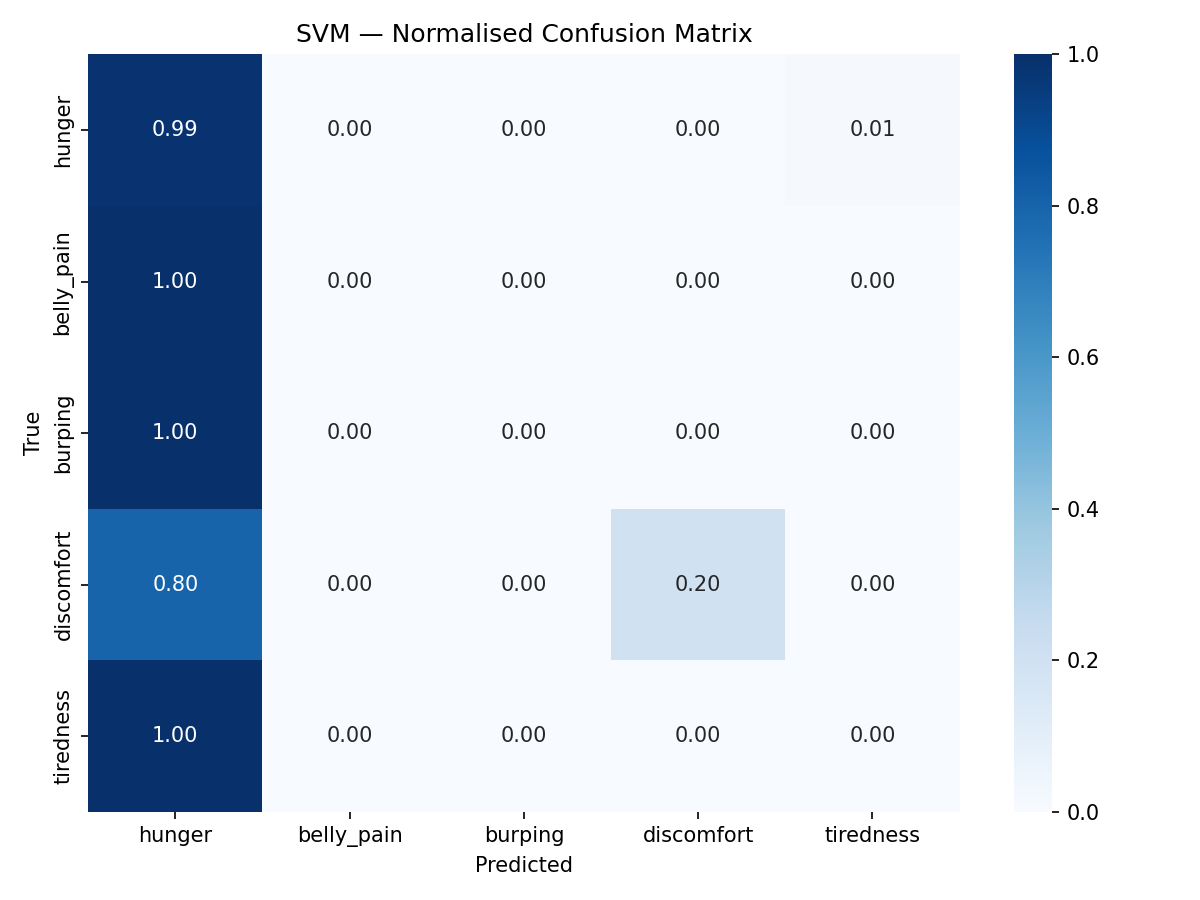
\includegraphics[width=0.48\textwidth]{../results/plots/SVM_confusion_matrix.png}
% \caption{Normalised confusion matrices for GMM (left) and SVM (right).}
% \end{figure}

\subsection{Statistical Checks}

\textit{(Stationarity and Gaussianity plots to be inserted from}
\texttt{results/plots/}\textit{.)}

% ======================================================================
\section{Discussion}
\label{sec:discussion}

\textit{(To be completed after results are available.)}

Key points to address:
\begin{itemize}[nosep]
  \item Which classes are easiest/hardest to distinguish and why.
  \item How stationarity and Gaussianity assumptions hold in practice.
  \item Feature importance — which MFCCs and spectral descriptors
        contribute most.
  \item Limitations of the current feature set and model choices.
  \item Motivation for Phase~2 (deep learning on spectrograms).
\end{itemize}

% ======================================================================
\section{Conclusion}
\label{sec:conclusion}

This phase establishes a classical machine-learning baseline for
five-class infant cry classification using a 750-dimensional feature
vector derived from MFCCs, delta coefficients, and spectral descriptors.
A GMM generative classifier and an SVM discriminative classifier are
trained and evaluated, with an exploratory HMM capturing temporal
structure.  Statistical validation confirms that the distributional
assumptions of these models are broadly satisfied.

Phase~2 will introduce deep-learning models operating on Mel-spectrogram
representations, and Phase~3 will fuse the classical and deep-learning
approaches into a hybrid ensemble.

% ======================================================================
\bibliographystyle{ieeetr}

\begin{thebibliography}{10}

\bibitem{dunstan2006}
P.~Dunstan,
``Dunstan Baby Language,'' 2006.
\newblock \url{https://www.dunstanbaby.com}

\bibitem{ji2021review}
C.~Ji, T.~Mudiyanselage, Y.~Gao, and Y.~Pan,
``A review of infant cry analysis and classification,''
\textit{EURASIP Journal on Audio, Speech, and Music Processing},
vol.~2021, no.~1, pp.~1--17, 2021.

\bibitem{chang2017infant}
C.-Y.~Chang and J.-J.~Li,
``Application of deep learning for recognizing infant cries,''
in \textit{Proc. IEEE Int. Conf. Consumer Electronics -- Taiwan
(ICCE-TW)}, pp.~53--54, 2017.

\bibitem{davis1980mfcc}
S.~Davis and P.~Mermelstein,
``Comparison of parametric representations for monosyllabic word
recognition in continuously spoken sentences,''
\textit{IEEE Transactions on Acoustics, Speech, and Signal Processing},
vol.~28, no.~4, pp.~357--366, 1980.

\bibitem{reynolds2000speaker}
D.~A.~Reynolds, T.~F.~Quatieri, and R.~B.~Dunn,
``Speaker verification using adapted Gaussian mixture models,''
\textit{Digital Signal Processing}, vol.~10, no.~1--3, pp.~19--41, 2000.

\bibitem{chang2011libsvm}
C.-C.~Chang and C.-J.~Lin,
``LIBSVM: A library for support vector machines,''
\textit{ACM Transactions on Intelligent Systems and Technology},
vol.~2, no.~3, pp.~1--27, 2011.

\bibitem{rabiner1989hmm}
L.~R.~Rabiner,
``A tutorial on hidden Markov models and selected applications in
speech recognition,''
\textit{Proceedings of the IEEE}, vol.~77, no.~2, pp.~257--286, 1989.

\bibitem{hershey2017cnn}
S.~Hershey \textit{et al.},
``CNN architectures for large-scale audio classification,''
in \textit{Proc. IEEE ICASSP}, pp.~131--135, 2017.

\end{thebibliography}

\end{document}
